\documentclass[border=8pt]{standalone}
\usepackage{amsmath}
\usepackage{tikz}
\usetikzlibrary{arrows.meta,positioning,calc}
\begin{document}
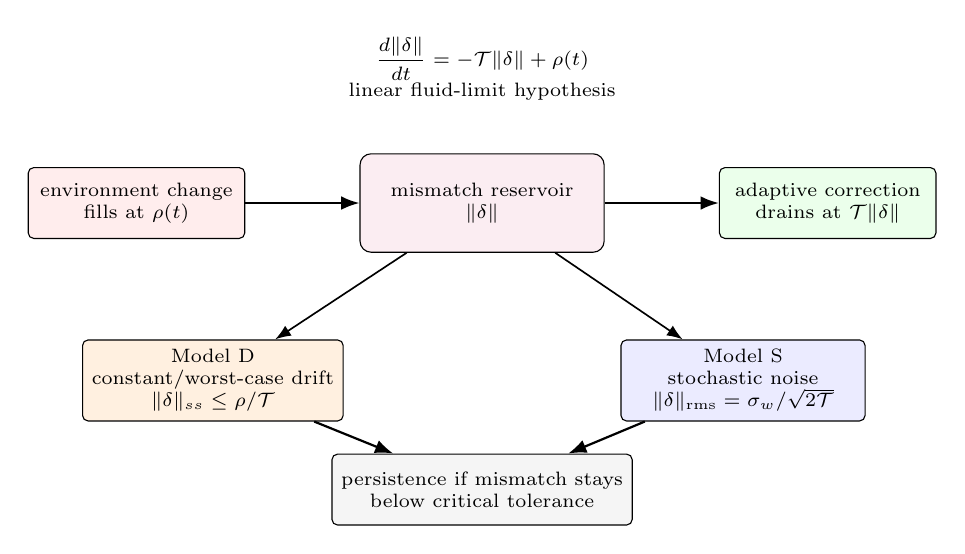
\begin{tikzpicture}[
  box/.style={draw, rounded corners=2pt, align=center, minimum width=2.75cm, minimum height=0.9cm, font=\scriptsize},
  tank/.style={draw, rounded corners=4pt, align=center, minimum width=3.1cm, minimum height=1.25cm, font=\scriptsize, fill=purple!7},
  note/.style={align=center, font=\scriptsize},
  arr/.style={-Latex, thick},
  thinarr/.style={-Latex, semithick}
]

\node[tank] (mismatch) {mismatch reservoir\\$\|\delta\|$};
\node[box, fill=red!7, left=1.45cm of mismatch] (dist) {environment change\\fills at $\rho(t)$};
\node[box, fill=green!8, right=1.45cm of mismatch] (corr) {adaptive correction\\drains at $\mathcal T\|\delta\|$};

\draw[arr] (dist) -- (mismatch);
\draw[arr] (mismatch) -- (corr);

\node[box, fill=orange!12, below left=1.1cm and 0.2cm of mismatch, minimum width=3.1cm] (det)
  {Model D\\constant/worst-case drift\\$\|\delta\|_{ss}\leq\rho/\mathcal T$};
\node[box, fill=blue!8, below right=1.1cm and 0.2cm of mismatch, minimum width=3.1cm] (sto)
  {Model S\\stochastic noise\\$\|\delta\|_{\rm rms}=\sigma_w/\sqrt{2\mathcal T}$};
\draw[thinarr] (mismatch) -- (det);
\draw[thinarr] (mismatch) -- (sto);

\node[box, fill=gray!8, below=2.55cm of mismatch, minimum width=3.6cm] (threshold)
  {persistence if mismatch stays\\below critical tolerance};
\draw[arr] (det) -- (threshold);
\draw[arr] (sto) -- (threshold);

\node[note, above=0.55cm of mismatch] {$\dfrac{d\|\delta\|}{dt}=-\mathcal T\|\delta\|+\rho(t)$\\linear fluid-limit hypothesis};

\end{tikzpicture}
\end{document}
